\chapter{Sample Exam Paper 1}
\section{Question 1}
\textit{A manufacturer makes 1,000,000 chips per year, using a 1.5 Watt machine. Each chip takes 10 minutes to make, and energy is currently priced at \pounds 0.60 per Watt-hour. A new process would reduce the unit production time by 1 minute and energy consumption by 50\%. If all other costs remain the same, what is the maximum amount of money you would pay for this new process? Assume that the new process must pay for itself by the end of the first year.}

\textbf{5 marks}

Old process:
\begin{gather}
    \SI{10e6}{\minute}\times \frac{1}{60} = \SI{166666.67}{\hour}\\
    \SI{166666.67}{\hour} \times \SI{1.5}{\watt} = \SI{250000}{\watt\hour}\\
    \SI{250000}{\watt\hour} \times \SI{0.6}{\pounds} = \SI{150000}{\pounds}
\end{gather}
New process:
\begin{gather}
    \SI{9e6}{\minute}\times \frac{1}{60} = \SI{150000}{\hour}\\
    \SI{150000}{\hour} \times \SI{0.75}{\watt} = \SI{112500}{\watt\hour}\\
    \SI{112500}{\watt\hour} \times \SI{0.6}{\pounds} = \SI{67500}{\pounds}
\end{gather}
Maximum amount that should be paid:
\begin{gather}
    \SI{150000}{\pounds} - \SI{67500}{\pounds} = \SI{82500}{\pounds}
\end{gather}
\section{Question 2}
\textit{Two mutually exclusive investment alternatives are being considered by an automotive engineering manufacturer, and one of them must be selected. Alternative A requires an initial investment of \pounds 13,000 in equipment. Annual operating and maintenance costs are anticipated to be normally distributed, with a mean of \pounds 5,000 and a standard deviation of \pounds 500. The terminal salvage value at the end of the eight-year planning horizon is anticipated to be normally distributed, with a mean of \pounds 2,000 and a standard deviation of \pounds 800. Alternative B requires end-of-year annual expenditures over the eight-year planning horizon, with the annual expenditure being normally distributed with a mean of \pounds 7,500 and a standard deviation of \pounds 750. Using a MARR of 15\% per year, what is the probability that Alternative A is the most economic alternative (i.e., the least costly)?}

Hint: The addition or subtraction of two normally distributed random variables is a normally distributed random variable.

\textbf{25 marks}

\begin{table}[H]
    \centering
    \begin{tabular}{@{}llllll@{}}
        \toprule
        Alternative A &                   &                 & Alternative B &                   &                 \\
        \midrule
        Initial costs & \pounds 13000     &                 & Annual O\&M   & \pounds 7500 mean & \pounds 750 STD \\
        Annual O\&M   & \pounds 5000 mean & \pounds 500 STD &               &                   &                 \\
        Salvage value & \pounds 2000 mean & \pounds 800 STD &               &                   &                 \\
        \bottomrule
    \end{tabular}
\end{table}
Mean NPV Alternative A:
\begin{gather}
    -13000 - 5000\times \frac{\left(1.15\right)^8 - 1}{0.15\left(1.15\right)^8} + 2000\times \frac{1}{1.15^8} = -34782.80 \pounds
\end{gather}
Variance of NPV Alternative A:
\begin{gather}
    500^2 \sum_{k=1}^8 \frac{1}{1.15^{2k}} + 800^2 \times \frac{1}{1.15^16} = 760746\pounds^2
\end{gather}
Mean NPV Alternative B
\begin{gather}
    -7500\times \frac{\left(1.15\right)^8 - 1}{0.15\left(1.15\right)^8} = -33655\pounds
\end{gather}
Variance of NPV Alternative B
\begin{gather}
    750^2\sum_{k=1}^8 \frac{1}{1.15^{2k}} = 1557794\pounds^2
\end{gather}
\section{Question 3}
\textit{The tree diagram in Figure 1 describes the uncertain cash flows for an engineering project. The analysis period is two years (as shown in Figure \ref{fig:dt1}) and MARR = 15\% per year.}
\begin{figure}[H]
    \centering
    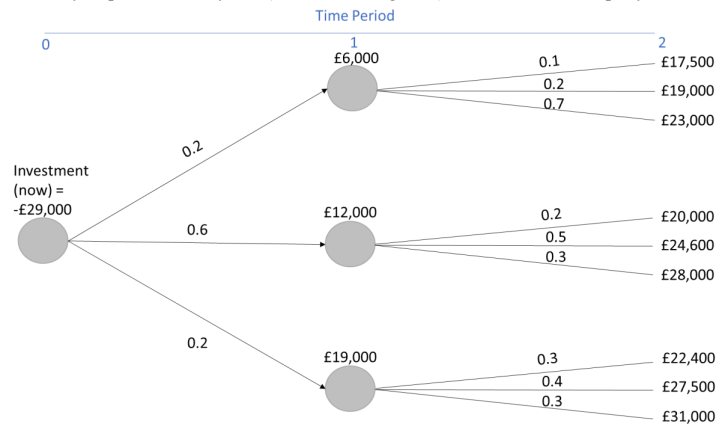
\includegraphics[width = 0.9\textwidth]{img/figure65.png}
    \caption{Decision tree for Question 3. The time period is measured in years and represents the end of the corresponding year.}
    \label{fig:dt1}
\end{figure}
\textit{What is the average, variance and standard deviation of NPV?}

\textbf{25 marks}

From the decision tree, it can be observed that there are nine possible values of NPV, calculated as follows:
\begin{align}
    (1) & \qquad -29000 + \frac{6000}{1.15} + \frac{17500}{1.15^2} = -10551 \qquad & p(1) = 0.02 \\
    (2) & \qquad -29000 + \frac{6000}{1.15} + \frac{19000}{1.15^2} = -9417 \qquad  & p(2) = 0.04 \\
    (3) & \qquad -29000 + \frac{6000}{1.15} + \frac{23000}{1.15^2} = -6392 \qquad  & p(3) = 0.14 \\
    (4) & \qquad -29000 + \frac{12000}{1.15} + \frac{20000}{1.15^2} = -3443 \qquad & p(4) = 0.12 \\
    (5) & \qquad -29000 + \frac{12000}{1.15} + \frac{24600}{1.15^2} = 35 \qquad    & p(5) = 0.30 \\
    (6) & \qquad -29000 + \frac{12000}{1.15} + \frac{28000}{1.15^2} = 2606 \qquad  & p(6) = 0.18 \\
    (7) & \qquad -29000 + \frac{19000}{1.15} + \frac{22400}{1.15^2} = 4459 \qquad  & p(7) = 0.06 \\
    (8) & \qquad -29000 + \frac{19000}{1.15} + \frac{27500}{1.15^2} = 8315 \qquad  & p(8) = 0.08 \\
    (9) & \qquad -29000 + \frac{19000}{1.15} + \frac{31000}{1.15^2} = 10962 \qquad & p(9) = 0.06
\end{align}
We know that:
\begin{align}
    E\left(X\right) & = \sum x_i p\left(x_i\right)                                  \\
    V\left(X\right) & = \sum \left[x_i - E\left(x\right)\right]^2 p\left(x_i\right)
\end{align}
Thus average is:
\begin{multline}
    E\left(NPV\right) = \left(-10551 \times 0.02\right) + \left(-9417 \times 0.04\right) + \left(-6392 \times 0.14\right) + \left(-3443 \times 0.12\right) + \left(35 \times 0.30\right) + \\ \left(2606 \times 0.18\right) + \left(4459 \times 0.06\right) + \left(8315 \times 0.08\right) + \left(10962 \times 0.06\right)
\end{multline}
\begin{equation}
    E\left(NPV\right) = \SI{175}{\pounds}
\end{equation}
Variance:
\begin{multline}
    V\left(NPV\right) = \left(\left(-10551 -175\right)^2\times 0.02 \right) +
    \left(\left(-9417 -175\right)^2\times 0.04 \right) +
    \left(\left(-6932 -175\right)^2\times 0.14 \right) +\\
    \left(\left(-3443 -175\right)^2\times 0.12 \right) +
    \left(\left(35 -175\right)^2\times 0.30 \right) +
    \left(\left(2606 -175\right)^2\times 0.18 \right) + \\
    \left(\left(4459 -175\right)^2\times 0.06 \right) +
    \left(\left(8315 -175\right)^2\times 0.08 \right) +
    \left(\left(10962 -175\right)^2\times 0.06 \right)
\end{multline}
\begin{equation}
    V\left(NPV\right) = \SI{29.04e6}{\pounds^2}
\end{equation}
Standard deviation:
\begin{gather}
    SD\left(NPV\right) = \sqrt{V\left(NPV\right)} = \sqrt{\SI{29.04e6}{}} = \SI{5295}{\pounds}
\end{gather}
\textit{What is the probability that NPV $<$ 0?}

\textbf{5 marks}

The probability that NPV $<$ 0 is the sum of the probabilities associated with negative values of NPV:
\begin{gather}
    P\left(NPV < 0\right) = 0.02 + 0.04 + 0.14 + 0.12 = 0.32
\end{gather}
\section{Question 4}
UCL Engineering plc is a multinational engineering equipment trader and distribution company that has been established for many years. Its income and balance sheet for two years are provided in Table \ref{tab:incStat1} and Table \ref{tab:balSheet1} respectively.
\begin{table}[H]
    \centering
    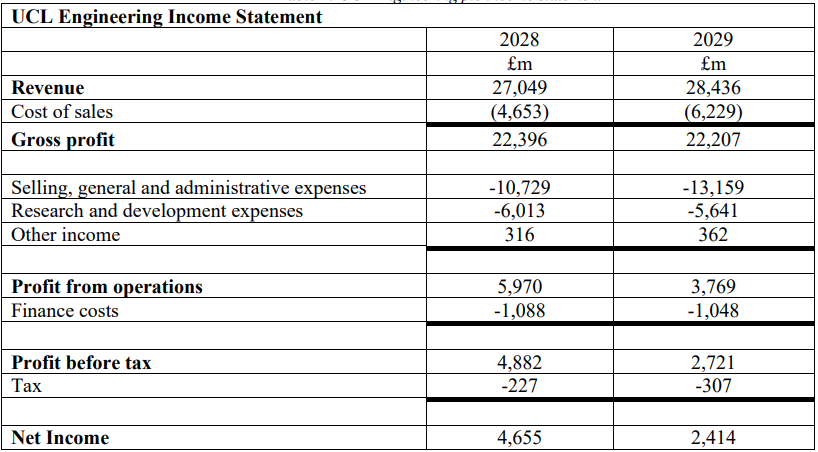
\includegraphics[width = 0.9\textwidth]{img/figure66.png}
    \caption{UCL Engineering plc income statement.}
    \label{tab:incStat1}
\end{table}
\begin{table}[H]
    \centering
    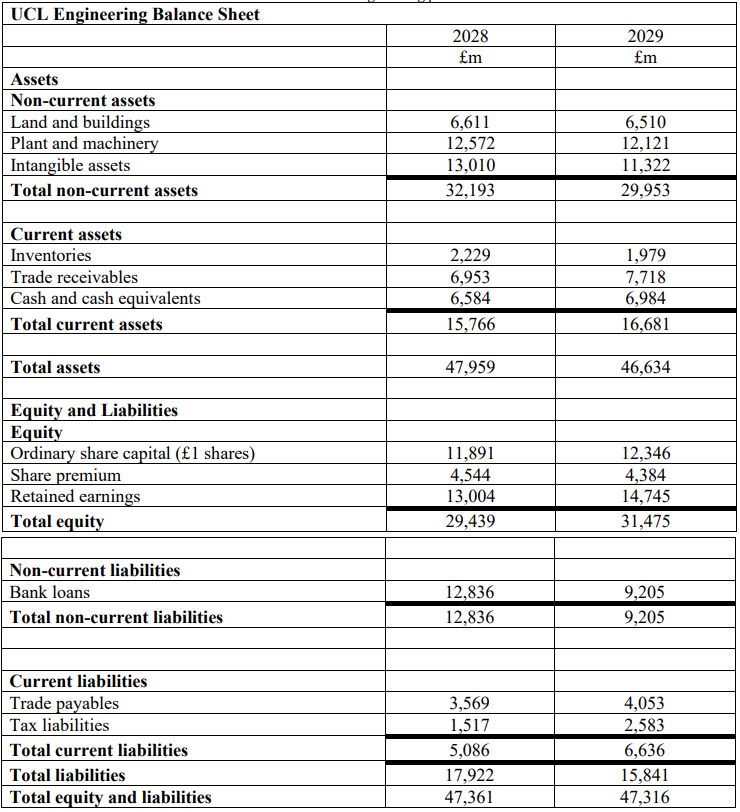
\includegraphics[width = 0.7\textwidth]{img/figure67.png}
    \caption{UCL Engineering plc balance sheet.  Note the inventory for the company in 2027 is valued at \pounds 2,450 million.}
    \label{tab:balSheet1}
\end{table}
\newpage
\textit{Explain the terms ``gross profit'', ``non-current assets'' and ``current liabilities'' that feature in either the Income Statement or the Balance Sheet.}

\textbf{10 marks}
\begin{itemize}
    \item Gross profit is the income generated from sales, minus the costs of selling the goods. It also accounts for expenses like general expenses and taxes that need to be subtracted to find net income.
    \item Non-current assets are a company's long-term (economic) obligations listed on the balance sheet. Long-term refers to assets that are not expected to be converted to cash over the next one-year period.
    \item Current liabilities are a company's short term (economic) obligations, due within a one year period.
\end{itemize}
\textit{Calculate the financial ratios shown in Table \ref{tab:finRatio1} and use them to provide a one-paragraph interpretation of the company's general performance.}

\textbf{30 marks}
\begin{table}[H]
    \centering
    \begin{adjustbox}{max width=\textwidth}
        \begin{tabular}{@{}lcccc@{}}
            \toprule
                                       & \textbf{Formula}                                                                     & \textbf{2028}                         & \textbf{2029}                         & \textbf{Industry average} \\
            \midrule
            \addlinespace[0.5em]
            Current ratio              & $\dfrac{\textrm{Current assets}}{\textrm{Current liabilities}}$                      & $\dfrac{15766}{5086} = 3.09$          & $\dfrac{16681}{6636} = 2.51$          & 2.2                       \\
            \addlinespace[1em]
            Quick ratio                & $\dfrac{\textrm{Current assets} - \textrm{Inventory}}{\textrm{Current liabilities}}$ & $\dfrac{15766 - 2229}{5086} = 2.66$   & $\dfrac{16681 - 1979}{6636} = 2.66$   & 1.6                       \\
            \addlinespace[1em]
            Debt-Equity ratio          & $\dfrac{\textrm{Total liabilities}}{\textrm{Total equity}}$                          & $\dfrac{17922}{29439} = 0.61$         & $\dfrac{15841}{31475} = 0.50$         & 37.38\%                   \\
            \addlinespace[1em]
            Inventory turnover         & $\dfrac{\textrm{Cost of sales}}{\textrm{Average inventory}}$                         & $\dfrac{4653}{0.5(2229+2450)} = 1.99$ & $\dfrac{6229}{0.5(2229+1979)} = 2.96$ & 2.99                      \\
            \addlinespace[1em]
            Day sales in inventory     & $\dfrac{365}{\textrm{Inventory turnover}}$                                           & $\dfrac{365}{1.99} = 183.87$          & $\dfrac{365}{2.96} = 123.29$          & 1.3                       \\
            \addlinespace[1em]
            Total asset turnover ratio & $\dfrac{\textrm{Total annual sales}}{\textrm{Total assets}}$                         & $\dfrac{27049}{47959} = 0.56$         & $\dfrac{28436}{46634} = 0.61$         & 0.81                      \\
            \addlinespace[1em]
            Profit margin              & $\dfrac{\textrm{Net income}}{\textrm{Net sales}}$                                    & $\dfrac{4655}{27049} = 0.17$          & $\dfrac{2414}{28436} = 0.08$          & 8.3\%                     \\
            \addlinespace[1em]
            Return on assets ratio     & $\dfrac{\textrm{Net income}}{\textrm{Total assets}}$                                 & $\dfrac{4655}{47959} = 0.10$          & $\dfrac{2414}{46634} = 0.05$          & 5.2\%                     \\
            \addlinespace[1em]
            Return on equity ratio     & $\dfrac{\textrm{Net income}}{\textrm{Total equity}}$                                 & $\dfrac{4655}{29439} = 0.16$          & $\dfrac{2414}{31475} = 0.08$          & 2.1\%                     \\
            \addlinespace[0.5em]
            \bottomrule
        \end{tabular}
    \end{adjustbox}
    \caption{Financial ratios and their industry average values for Question 4.}
    \label{tab:finRatio1}
\end{table}
In comparison to industry averages, the company's financial performance exhibits both strengths and weaknesses. In terms of liquidity, the company surpasses the industry average with a current ratio of 3.09 in 2028 and 2.51 in 2029, above the standard of 2.2, indicating a healthier ability to meet short-term obligations. However, the company poses a higher risk for shareholders than the industry standard, as evidenced by a debt-equity ratio surpassing the 50\% mark in both years, significantly higher than the average of 37.38\%.

In 2028, the company's inventory turnover nearly matches the industry average, although its day sales in inventory and total asset turnover ratio, at 183.87 and 0.56 respectively, suggest less efficiency in converting inventory and assets into sales compared to the average industry values of 1.3 and 0.81.

Profitability, however, presents a mixed picture. The company showed superior profitability in 2027, but by 2028, its profit margin regressed to the industry average of 8.3\%. While the return on assets ratio approximated the industry average, the return on equity ratio was notably higher, indicating a better-than-average efficiency at converting equity into profits.

Comparing the company's performance between the years 2028 and 2029, a general decline in liquidity is observed, indicated by the decrease in both the current and quick ratios. Conversely, there is a reduction in shareholder risk, as shown by the lowered debt-equity ratio in 2029. Additionally, the company has shown improvement in asset efficiency, as suggested by the increased inventory turnover and total asset turnover ratio. However, profitability shows a general decline, with profit margin and return on both assets and equity witnessing a drop in 2029.